\documentclass[11pt,a4paper,twocolumn]{article}

% === Core Packages ===
\usepackage[margin=2cm]{geometry}
\usepackage[utf8]{inputenc}
\usepackage[T1]{fontenc}
\usepackage{times}
\usepackage{amsmath,amssymb}
\usepackage{graphicx}
\usepackage{booktabs}
\usepackage{float}
\usepackage{enumitem}
\usepackage{tikz}
\usepackage{pgfplots}
\pgfplotsset{compat=1.18}
\usetikzlibrary{arrows.meta,shapes.geometric,positioning,calc,decorations.markings,fit,backgrounds}

% === Citation (IEEE style) ===
\usepackage[numbers,sort&compress]{natbib}
\bibliographystyle{IEEEtranN}

% === Hyperref ===
\usepackage[hidelinks]{hyperref}
\usepackage{xurl}

% === Settings ===
\setlength{\parindent}{1em}
\setlength{\parskip}{0.3em}

% === Title ===
\title{\textbf{Decentralizēts reputācijas tīkls:\\ietvars sabiedrības dabiskai organizācijai}}
\author{Pavel Kudrna\\Prague, Czechia\\Draft v1 --- March 2026}
\date{}

\begin{document}
\maketitle

% ============================================================
% ABSTRACT
% ============================================================
\begin{abstract}
Taisnīguma izjūta---pārliecība, ka netaisnības tiek labotas un nopelni atalgoti---ir spēcīgākais sabiedrības saliedēšanas spēks. Kad centralizētas pārvaldes institūcijas nespēj šo izjūtu nodrošināt, jo tiesību aizstāvēšanas izmaksas pārsniedz pašas tiesības vērtību, sabiedrības saliedētība kļūst vājāka. Pašreizējās institucionālās struktūras neatrisina nozīmīgu strīdu kategoriju sistemātiski tāpat, kā centrālā plānošana nespēj sadalīt resursus: caur informācijas asimetriju, trūkstošām atgriezeniskās saites cilpām un lēmumu pieņēmēju atrautību no savu lēmumu sekām. Šajā rakstā tiek prezentēts reputācijas sociālais tīkls (RSN): decentralizēts, nepiekukuļojams, cenzūrai izturīgs komunikācijas slānis, kas balstīts uz decentralizētiem identifikatoriem (DID) un kas ļauj pseidonīmiem dalībniekiem publicēt, verificēt un patērēt reputācijas informāciju par reālās pasaules uzvedību. Pamatmehānisms balstās uz trim projektēšanas principiem: (1)~asimetriska izmaksu struktūra, kurā reputācijas datu lasīšana ir lēta, bet rakstīšanai nepieciešams verificējams pūliņš; (2)~nedeterministisks verificētāju atlases protokols, kas balstīts uz konsekventu jaukšanu un kas rada radikālu apgalvojumu cenu caur pieaugošām iterāciju izmaksām; un (3)~uz tirgu balstīts reputācijas autoritātes modelis, kurā privātie verificētāji ieliek uz spēles savu uzkrāto reputāciju par to apgalvojumu precizitāti, ko tie apstiprina. Iegūtā arhitektūra rada emerģentu meritokrātiju bez centrālas koordinācijas un dara iespējamu pakāpenisku, atgriezenisku migrācijas ceļu no esošajām valsts pārvaldītajām sistēmām.
\end{abstract}

% ============================================================
% 1. INTRODUCTION
% ============================================================
\section{Ievads}

\subsection{Centralizētas uzticēšanās problēma}

Mūsdienu pārvalde balstās uz fundamentālu pieņēmumu: ka centralizētas institūcijas var starpniekot uzticēšanos starp svešiniekiem lielā mērogā. Tiesas izšķir strīdus. Reģistri apliecina īpašumtiesības. Regulatīvās iestādes uzrauga standartu ievērošanu. Šīs institūcijas tika izveidotas laikmetā, kad informācija bija reta, komunikācija lēna un pilnvaru deleģēšana centrālajai institūcijai bija vienīgais iespējamais koordinācijas mehānisms. Tomēr centralizēta pārvalde neizdodas to pašu strukturālo iemeslu dēļ kā centrālā plānošana: informācijas asimetrija, trūkstošas atgriezeniskās saites cilpas un lēmumu pieņēmēju atrautība no savu lēmumu sekām.

Pieņēmums neizdodas, piemēram, tad, kad institucionālās starpniecības izmaksas pārsniedz strīda vērtību. Iedomāsimies īrnieku, kurš atklāj, ka viņa īrētajam dzīvoklim trūkst likumā prasītā elektrodrošības sertifikāta---apstākļa, kas rada tūlītējus draudus dzīvībai. Īrnieka juridiskās tiesības atkāpties no līguma ir nepārprotamas. Tomēr šo tiesību aizstāvēšanas izmaksas caur tiesu sistēmu pārsniedz drošības naudas un pienākošos zaudējumu naudisko vērtību, pat ieskaitot iespējamo likumā noteikto kompensāciju~\cite{czcourtfees}. Racionālā atbilde ir zaudējumu absorbēt un aiziet.

Šis nav patoloģisks izņēmuma gadījums. Tā ir noklusētā pieredze nozīmīgai strīdu kategorijai, kurā kaitējums ir reāls, bet naudiskā likme ir zem sliekšņa, no kura institucionālā aizstāvēšana kļūst ekonomiski racionāla. Rezultāts ir sistēma, kas strukturāli dod priekšroku ļaunprātīgiem dalībniekiem: tie, kas kaitē citiem apjomos zem šī sliekšņa, var rīkoties nesodīti, jo taisnīguma meklēšanas izmaksas gulstas uz cietušo pusi.

Iepriekšējais piemērs ir ņemts no autora tiesiskās vides---Čehijas civiltiesību sistēmas. Citās tiesību tradīcijās---uz precedentiem balstītajās vispārējās tiesībās, paražu tiesībās, jauktās sistēmās---taisnīgums neizdodas dažādos veidos un dažādā mērā atkarībā no jurisdikcijas kultūras un procesuālajām īpatnībām. Lasītāji, visticamāk, atpazīs līdzvērtīgus piemērus no sava konteksta. Strukturāli universāls ir šis raksts: strīdi, kuru vērtība ir zem ekonomiski racionālas aizstāvēšanas sliekšņa, beidzas ar to, ka zaudējumu absorbē cietusī puse. RSN nesola perfektu taisnīgumu---tas tikai samazina strukturālo priekšrocību, kādu ļaunprātīgi dalībnieki bauda tad, kad institucionālā aizstāvēšana ir ekonomiski neizdevīga.

\subsection{Kāpēc esošie risinājumi ir nepietiekami}

\textbf{Decentralizētas identitātes (DID) ietvari}~\cite{did2022} nodrošina kriptogrāfiskus mehānismus paš\-suverēnai identitātes pārvaldībai, taču koncentrējas galvenokārt uz identitātes verifikāciju, neaptverot plašāko uzvedības reputācijas jautājumu.

\textbf{Ar dvēseli saistītie žetoni (SBT)}~\cite{weyl2022} fiksē ieskatu, ka reputācija nav pārnesama, taču balstās uz blokķēdes infrastruktūru ar mērogošanas ierobežojumiem un neaptver ekonomiskos stimulus, kas pārvalda informācijas ievadi. Radniecīgi jēdzieni, piemēram, nopelnu žetoni (piem., Liberland), balstās uz līdzīgu filozofiju, taču paliek piesaistīti konkrētiem jurisdikcijas ietvariem.

\textbf{Decentralizētas autonomas organizācijas (DAO)}~\cite{buterin2014} īsteno pārvaldi caur viedlīgumiem, taču atkārto plutokrātisku dinamiku, kurā ietekme ir proporcionāla kapitālam. Kvadrātiskā balsošana~\cite{buterin2019} to daļēji mazina, taču ierobežo praktisko ieviešanu. DAO saskaras arī ar fundamentālo \emph{orākula problēmu}: viedlīgumi nespēj uzticami verificēt reālās pasaules stāvokļus bez uzticama ārēja avota, un šai problēmai blokķēdes arhitektūrā nav vispārēja risinājuma.

Neviena esošā sistēma neapvieno decentralizāciju, izturību pret cenzūru, pseidonimitāti, verificējamas ievades izmaksas un emerģentu konsensu.

\subsection{Ieguldījums}

Šis raksts sniedz šādu ieguldījumu:
\begin{enumerate}[nosep]
\item \textbf{Reputācijas sociālā tīkla (RSN)} definīciju---decentralizēta protokola, kas paplašina DID ietvaru, lai atbalstītu divpusēju reputācijas apmaiņu.
\item \textbf{Nedeterministisku verificētāju atlases protokolu}, kas balstīts uz konsekventu jaukšanu~\cite{karger1997}.
\item \textbf{Dārgā radikālisma principu}, kas cenas apgalvojumus atbilstoši to attālumam no tīkla konsensa caur trim savstarpēji pastiprinošiem izmaksu kanāliem.
\item \textbf{Reputablas autoritātes modeli} ar asimetriskiem stimuliem, kur nepatiess apstiprinājums izmaksā katastrofāli vairāk nekā leģitīmas maksas.
\item \textbf{Pakāpenisku migrācijas ceļu} caur paralēlu fiskālo infrastruktūru.
\end{enumerate}

% ============================================================
% 2. DESIGN PRINCIPLES
% ============================================================
\section{Projektēšanas principi}

RSN arhitektūru ierobežo pieci nepārkāpjami projektēšanas principi.

\textbf{Nepārtrauktība un evolūcija.} Sistēma līdzāspastāv ar esošajām institūcijām nenoteikta ilguma pārejas periodā. Pārejai jābūt atgriezeniskai katrā posmā.

\textbf{Brīvprātība un atbildība.} Dalība ir brīvprātīga, taču brīvprātība ir savienota ar atbildību: dalībnieks, kurš uzņemas kontroli pār institucionālu funkciju, vienlaikus uzņemas arī tai pievienotās saistības.

\textbf{Daudzveidība un kultūras neitralitāte.} Konsenss rodas no divpusējām mijiedarbībām, nevis no sistēmas projektētāju uzspiestiem iepriekš noteiktiem noteikumiem.

\textbf{Noturība un izturība pret cenzūru.} Tīkla cenzēšanas izmaksām jāpārsniedz tā paciešanas izmaksas. Tikai pilnīgs totalitārisms---par postošu politisku un ekonomisku cenu---var sistēmu apspiest.

\textbf{Konsenss un piespiešana.} Sistēma iekļauj cilvēka tieksmes uz sīkumainību, ļaunprātību un atriebīgu gandarījumu kā nesošas iezīmes. Nekrietnība nav aizliegta; tā tiek cenota.

% ============================================================
% 3. SYSTEM OVERVIEW
% ============================================================
\section{Sistēmas pārskats}

\subsection{Reputācijas sociālais tīkls}

RSN ir decentralizēts, vienādranga (peer-to-peer) komunikācijas slānis, kurā dalībnieki apmainās ar verificējamu informāciju par reālās pasaules uzvedību. Tā noteicošās īpašības ir: decentralizēta un cenzējama neesoša infrastruktūra; pseidonīma dalība caur DID; asimetriska izmaksu struktūra (lasīšana ir lēta, rakstīšana dārga); kriptogrāfiska verificējamība; un \textbf{standartu atbalsts}---mašīnlasāmi formāti informācijai, kas tiek izplatīta tīklā, autoritāšu piedāvātajiem pakalpojumiem (apgalvojumu sastādīšana, apstiprināšana, liecinieka pakalpojums), kā arī politikas formātam, ieskaitot noteikumus otras puses reputācijas novērtēšanai un politikas neatbilstības riska novērtēšanai (starp deklarēto un faktisko uzvedību).

\subsection{Arhitektūras komponenti}

RSN sastāv no četriem galvenajiem komponentiem (att.~\ref{fig:architecture}):
\begin{enumerate}[nosep]
\item \textbf{DID slānis.} Dalībnieku identitātes ar deklarētiem noteikumiem, reputācijas metadatiem un tīkla maršrutēšanu.
\item \textbf{Apgalvojumu protokols.} Strukturēts formāts apgalvojumu par reālās pasaules notikumiem publicēšanai.
\item \textbf{Verifikācijas tīkls.} Decentralizēts protokols verificētāju piešķiršanai, izmantojot konsekventu jaukšanu.
\item \textbf{Reputācijas agregācijas slānis.} Pakalpojumi, kas rada cilvēklasāmus reputācijas kopsavilkumus.
\end{enumerate}

\begin{figure}[ht]
\centering
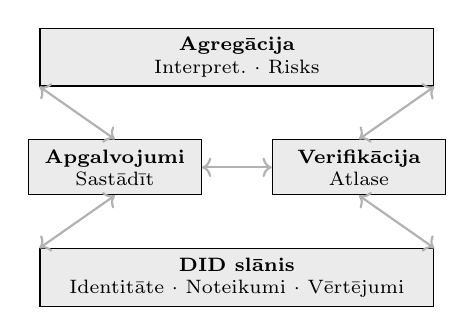
\begin{tikzpicture}[
    layer/.style={draw, minimum height=0.7cm, align=center, font=\scriptsize, fill=black!8},
    arr/.style={<->, thick, gray!60}
]
\node[layer, minimum width=5cm] (agg) at (0,2.8) {\textbf{Agregācija}\\Interpret.\ $\cdot$ Risks};
\node[layer, minimum width=2.2cm] (claim) at (-1.55,1.4) {\textbf{Apgalvojumi}\\Sastādīt};
\node[layer, minimum width=2.2cm] (verif) at (1.55,1.4) {\textbf{Verifikācija}\\Atlase};
\node[layer, minimum width=5cm] (did) at (0,0) {\textbf{DID slānis}\\Identitāte $\cdot$ Noteikumi $\cdot$ Vērtējumi};

\draw[arr] (agg.south west) -- (claim.north);
\draw[arr] (agg.south east) -- (verif.north);
\draw[arr] (claim.east) -- (verif.west);
\draw[arr] (claim.south) -- (did.north west);
\draw[arr] (verif.south) -- (did.north east);
\end{tikzpicture}
\caption{RSN četru slāņu arhitektūra.}
\label{fig:architecture}
\end{figure}

\subsection{Dalībnieku lomas}

Verifikācijas transakcijā ir iesaistītas līdz sešām atšķirīgām DID lomām (att.~\ref{fig:roles}): \textbf{Izdevējs} ($DID_I$, izveido un iesniedz apgalvojumu), \textbf{Subjekts} ($DID_S$, DID, par kuru ir apgalvojums---var sakrist ar Izdevēju), \textbf{Autoritāte} ($DID_A$, apstiprina apgalvojumu par maksu; var arī piedāvāt liecinieka pakalpojumus---\emph{izvēles}), \textbf{Liecinieks} ($DID_{W_{1..n}}$, inkognito verificētāja godīguma uzraugs caur izaicinājuma kodiem---\emph{izvēles}), \textbf{Verificētājs} ($DID_V$, algoritmiski atlasīts, lai publicētu apgalvojumu), un \textbf{RSN} (tīkls, kurā tiek publicēti verificētie apgalvojumi). Jebkuru lomu var deleģēt citam DID (7.4.\ sadaļa). Autoritāte parasti apvieno apstiprināšanu ar liecinieka pakalpojumiem, taču abas funkcijas ir loģiski neatkarīgas.

\begin{figure}[ht]
\centering
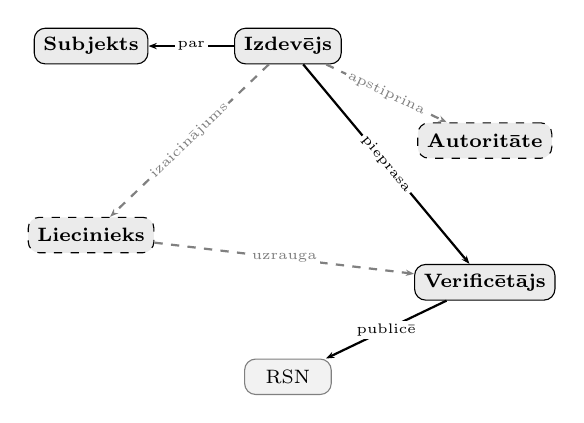
\begin{tikzpicture}[
    role/.style={draw, rounded corners, minimum width=1.1cm, minimum height=0.45cm, align=center, font=\scriptsize, fill=black!8},
    opt/.style={draw, rounded corners, minimum width=1.1cm, minimum height=0.45cm, align=center, font=\scriptsize, fill=black!8, dashed},
    arr/.style={-{Stealth[length=3pt]}, thick},
    oarr/.style={-{Stealth[length=3pt]}, thick, dashed, gray},
    lbl/.style={font=\tiny, fill=white, inner sep=1pt}
]
\node[role] (I) at (0,2.4) {\textbf{Izdevējs}};
\node[role] (S) at (-2.5,2.4) {\textbf{Subjekts}};
\node[opt] (A) at (2.5,1.2) {\textbf{Autoritāte}};
\node[opt] (W) at (-2.5,0) {\textbf{Liecinieks}};
\node[role] (V) at (2.5,-0.6) {\textbf{Verificētājs}};
\node[role, fill=black!5, draw=gray] (N) at (0,-1.8) {RSN};

\draw[arr] (I) -- node[lbl] {par} (S);
\draw[oarr] (I) -- node[lbl,sloped] {apstiprina} (A);
\draw[oarr] (I) -- node[lbl,sloped] {izaicinājums} (W);
\draw[arr] (I) -- node[lbl,sloped] {pieprasa} (V);
\draw[oarr] (W) -- node[lbl] {uzrauga} (V);
\draw[arr] (V) -- node[lbl] {publicē} (N);
\end{tikzpicture}
\caption{DID lomas verifikācijas transakcijā. Punktētas = izvēles (Autoritāte, Liecinieks).}
\label{fig:roles}
\end{figure}

\subsection{Nepiekukuļojamība: četri spēki}

RSN nepiekukuļojamība nerodas no viena mehānisma, bet no četriem vienlaicīgiem spēkiem. Neviens pats par sevi nav pietiekams; tikai to kombinācija padara mēģinājumu korumpēt ekonomiski neracionālu.

\textbf{Neparedzams mērķis.} Katra apgalvojuma verificētājs tiek atlasīts nedeterministiski caur konsekventu jaukšanu (5.3.\ sadaļa). Uzbrucējs nevar iepriekš iemērķēt konkrētu verificētāju kukuļošanai, jo verificētāja identitāte ir apgalvojuma satura un iepriekšējo iterāciju funkcija, nevis izdevēja izvēle.

\textbf{Reputācijas svira---lēna augšup, ātra lejup.} Reputāciju var iegūt tikai pakāpeniski, caur ilgstošu konsekventu uzvedību. Tomēr to var katastrofāli zaudēt vienā krāpnieciskā apstiprinājumā (6.2.\ sadaļa). Šī asimetrija nozīmē, ka gadu gaitā uzkrātu reputāciju var iznīcināt viens negodīgs apstiprinājums; optimālā stratēģija paliek noraidīt aizdomīgus apgalvojumus.

\textbf{Publisks solījums.} Katrs DID turētājs publiski deklarē savu politiku---mašīnlasāmu noteikumu kopu, kurus tas apņemas ievērot. Novirze starp deklarāciju un faktisko uzvedību ir atklājama un tiek cenota kā reputācijas pārkāpums, kas ir smagāks par pašu pamatpārkāpumu (7.3.\ sadaļa). Tāpēc liekulība ir dārgāka par tiešu negodīgumu.

\textbf{Tīkla uzbrukuma izmaksu asimetrija.} Tīkla cenzēšanas vai destabilizēšanas izmaksas aug nelineāri līdz ar tīkla lielumu un blīvumu, kamēr tā paciešanas izmaksas paliek nemainīgas. Lai cenzūra atmaksātos, centralizētam dalībniekam tā būtu jāpiemēro visā tīklā---prasot pasākumus, kas ir nesamērīgi ar jebkādu iedomājamu ieguvumu (10.\ sadaļa).

% ============================================================
% 4. DECENTRALIZED IDENTITY MODEL
% ============================================================
\section{Decentralizētas identitātes modelis}

\subsection{DID ar īpašām īpašībām}

RSN paplašina W3C DID Core specifikāciju~\cite{did2022} ar: \textbf{Deklarētiem noteikumiem} (mašīnlasāmas uzvedības saistības), \textbf{Reputācijas metadatiem} (agregēts uzvedības vērtējums) un \textbf{Tīkla maršrutēšanu} (maināma sīpola (onion) vārteja, kas nošķirta no stabilās pozīcijas gredzenā).

\subsection{Apgalvojuma dzīves cikls}

Apgalvojums iziet cauri sešiem posmiem (att.~\ref{fig:lifecycle}): sastādīšana, izvēles autoritātes apstiprinājums, verificētāja atlase caur konsekventu jaukšanu, verifikācijas lēmums (pieņemt vai noraidīt ar iterāciju), publicēšana un reputācijas atjaunināšana visām pusēm.

\begin{figure}[ht]
\centering
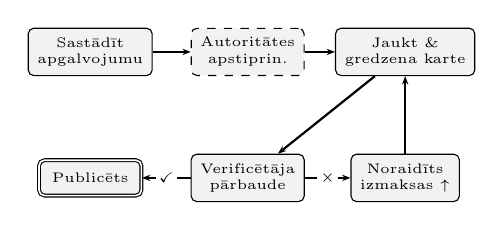
\begin{tikzpicture}[
    stp/.style={draw, rounded corners=2pt, minimum width=1.3cm, minimum height=0.45cm, align=center, font=\tiny, fill=black!5},
    arr/.style={-{Stealth[length=3pt]}, thick},
    lbl/.style={font=\tiny, fill=white, inner sep=1pt}
]
\node[stp] (comp) at (0,0) {Sastādīt\\apgalvojumu};
\node[stp, dashed] (auth) at (2.0,0) {Autoritātes\\apstiprin.};
\node[stp] (hash) at (4.0,0) {Jaukt \&\\gredzena karte};
\node[stp] (ver) at (2.0,-1.6) {Verificētāja\\pārbaude};
\node[stp, double] (pub) at (0,-1.6) {Publicēts};
\node[stp] (rej) at (4.0,-1.6) {Noraidīts\\izmaksas $\uparrow$};

\draw[arr] (comp) -- (auth);
\draw[arr] (auth) -- (hash);
\draw[arr] (hash) -- (ver);
\draw[arr] (ver) -- node[lbl] {\checkmark} (pub);
\draw[arr] (ver) -- node[lbl] {$\times$} (rej);
\draw[arr] (rej) -- ++(0,0.8) -| (hash);
\end{tikzpicture}
\caption{Apgalvojuma dzīves cikls ar iterāciju cilpu.}
\label{fig:lifecycle}
\end{figure}

\subsection{Saistība ar W3C DID Core}

RSN identitātes modelis ir W3C DID Core specifikācijas~\cite{did2022} īsts virskopums. Visi RSN DID ir derīgi W3C DID. RSN specifiskie paplašinājumi ir kodēti kā DID dokumenta īpašības, kas definētas atsevišķā DID metodes specifikācijā, saderīgā ar esošo infrastruktūru, piemēram, ION~\cite{buchner2021} un Ceramic~\cite{ceramic2023}.

% ============================================================
% 5. VERIFICATION AND PROPAGATION
% ============================================================
\section{Informācijas verifikācija un izplatīšana}

\subsection{Informācijas ievades izmaksas}

RSN pamata ekonomiskais princips ir asimetrija starp lasīšanu un rakstīšanu. Reputācijas datu lasīšana tuvojas nullei robežizmaksām dalībniekiem, kas ir daļa no DID tīkla un kam ir piekļuve, kas atbilst viņu reputācijai---jaunpienācējiem pakāpeniski jāizpelnās plašāka piekļuve (sk.\ pretpiesūkšanās mehānismu). Rakstīšana---saprasta kā reputācijas noturīga materializācija tīklā, nevis kā vienreizējs tehnisks akts---prasa verificējamu kumulatīvu ieguldījumu trijās dimensijās: \textbf{laiks} (dzīves gadi, kas pavadīti konsekventā uzvedībā, izpildītas saistības un koptas attiecības), \textbf{enerģija} (godīgā rīcībā ieguldītais pūliņš, rūpes par partnerībām un ilgtermiņa uzticamība) un \textbf{nauda} (ieguldījums savā vārdā---profesionālā izaugsme, sava darba kvalitāte, nodarītā kaitējuma atlīdzināšana). Reputāciju nevar nopirkt uzreiz---tā ir mūža uzkrājuma rezultāts, ko sistēma tikai padara redzamu un pārnesamu starp kontekstiem. Protokola vienreizējās tehniskās izmaksas (kriptogrāfiskie paraksti, verificētāju maksas) ir niecīgas salīdzinājumā ar šo pamatā esošo ieguldījumu.

\subsection{Sociālais grafs un kontaktu dziļums}

RSN pēc būtības ir sociāls tīkls: katrs DID pievieno kontaktus (citus DID), kas atļauj savienojumu. Šiem kontaktiem ir savi kontakti, un tā tālāk. Algoritmiskā verificētāju meklēšana darbojas konfigurējama dziļuma $h$ ietvaros starp saistītajiem kontaktiem (piem., $h=3$: cilvēka tiešie kontakti, viņu kontakti un kontaktu kontakti). Šī arhitektūra neprasa vienu globālu blokķēdi---tā dabiski atbalsta kopienu/klasteru rašanos ar pārklāšanos citās kopienās. Katram DID dalībniekam jābūt publicētai \textbf{politikai}---mašīnlasāmai noteikumu kopai, kas pārvalda, kā tiek novērtēti ienākošie pieprasījumi. Politikas pārkāpumi tiek reģistrēti tīklā kā negatīvi artefakti.

\subsection{Algoritmiskā verificētāju atlase}

Verifikācijas protokols izmanto konsekventu jaukšanu~\cite{karger1997} (att.~\ref{fig:verifier}). Verifikācija ir maksas pakalpojums: verificētāji darbojas par maksu, radot tirgu, kurā konkurence virza cenu veidošanu, ātrumu un uzticamību.

\textbf{1.\ solis.} Apgalvojuma dokuments tiek savienots ar iepriekšējās iterācijas jaukšanas rezultātu (vai $\varnothing$ pirmajā iterācijā) un jaukts:
\begin{equation}
\text{pos} = f_h(\text{claim} \| \text{prev\_hash})
\label{eq:hash}
\end{equation}

Algoritmam jāiekļauj visu iepriekšējo pieprasījumu un atbilžu \emph{pilnais ceļš}---ne tikai iepriekšējās iterācijas jaukšana. Katra verificētāja pilnā atbilde (pieņemšana, noraidīšana, kotētā cena, iemesls) tiek pievienota augošajam dokumentam, verificējama caur kriptogrāfiskiem parakstiem katrā solī.

\textbf{2.\ solis.} Jaukšana tiek attēlota uz $N$ pozīcijām konsekventā jaukšanas gredzenā, vienmērīgi sadalītām (piem., $N=4$ gadījumā: $+0^{\circ}, +90^{\circ}, +180^{\circ}, +270^{\circ}$). No katras pozīcijas pulksteņrādītāja virziena meklēšana izvēlas tuvāko DID kā verificētāja kandidātu (att.~\ref{fig:multipoint}). $N$ ir mainīgs parametrs, kas var būt atkarīgs no pašlaik aktīvo DID procentuālā daudzuma, diennakts laika vai tīkla vēsturiskās atsaucības.

\textbf{3.\ solis.} Verificētājs pieņem (publicē, liekot uz spēles reputāciju) vai noraida (atgriežoties pie 1.\ soļa ar noraidījuma jaukšanu). Kad mezgls neatbild, neskatoties uz deklarēto tiešsaistes statusu, nākamajam pieprasījumam jāiekļauj visas atbildes no visiem $N$ iepriekšējiem verificētāju kandidātiem.

\textbf{Pretpiesūkšanās.} Mērķa DID var noteikt maksas vai piekļuves ierobežojumus pieprasījumiem no jauniem DID ar nelielu reputāciju. Šis pakāpeniskais mehānisms (nevis binārs) piespiež jaunpienācējus veidot reputāciju caur patiesu aktivitāti, pirms tie brīvi patērē citu datus.

\begin{figure}[ht]
\centering
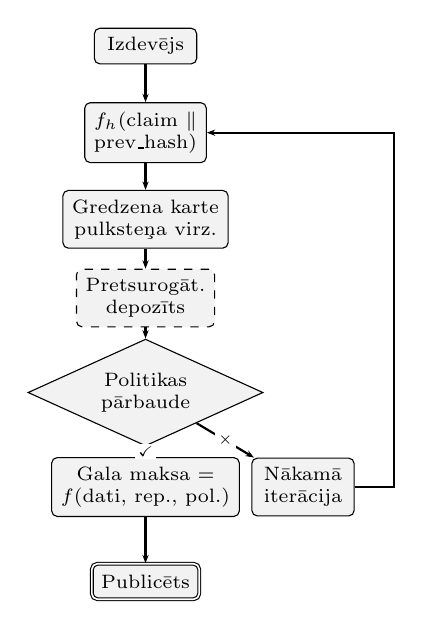
\begin{tikzpicture}[
    box/.style={draw, rounded corners=2pt, minimum width=1.3cm, minimum height=0.45cm, align=center, font=\scriptsize, fill=black!5},
    dec/.style={draw, diamond, aspect=2.2, minimum width=0.9cm, align=center, font=\scriptsize, fill=black!5},
    arr/.style={-{Stealth[length=3pt]}, thick},
    lbl/.style={font=\tiny, fill=white, inner sep=1pt}
]
\node[box] (iss) at (0,0) {Izdevējs};
\node[box] (hash) at (0,-1.1) {$f_h$(claim $\|$\\prev\_hash)};
\node[box] (ring) at (0,-2.2) {Gredzena karte\\pulksteņa virz.};
\node[box, dashed] (spam) at (0,-3.2) {Pretsurogāt.\\depozīts};
\node[dec] (check) at (0,-4.4) {Politikas\\pārbaude};
\node[box] (rej) at (2,-5.6) {Nākamā\\iterācija};
\node[box] (fee) at (0,-5.6) {Gala maksa =\\$f$(dati, rep., pol.)};
\node[box, double] (pub) at (0,-6.8) {Publicēts};

\draw[arr] (iss) -- (hash);
\draw[arr] (hash) -- (ring);
\draw[arr] (ring) -- (spam);
\draw[arr] (spam) -- (check);
\draw[arr] (check) -- node[lbl] {$\times$} (rej);
\draw[arr] (check) -- node[lbl] {\checkmark} (fee);
\draw[arr] (fee) -- (pub);
\draw[arr] (rej.east) -- ++(0.5,0) |- (hash.east);
\end{tikzpicture}
\caption{Verificētāju atlases protokols. Pretsurogāta depozīts ir izvēles un var būt atmaksājams. Gala maksu maksā tikai pēc pieņemšanas.}
\label{fig:verifier}
\end{figure}

Katrs noraidījums pievieno verificētāja pilno atbildi (ieskaitot iemeslus un nosacījumus) apgalvojuma dokumentam, paplašinot tā saturu. No paplašinātā dokumenta nedeterministiski tiek aprēķināta jauna jaukšana, kas attēlojas uz citu gredzena pozīciju un izvēlas citu verificētāju. Pilnā ceļa dokumentēšana ir obligāta---izdevējs nevar paredzēt vai ietekmēt nākamo verificētāju. Ja verificētājs ignorē pieprasījumu, neskatoties uz saderīgu deklarēto politiku, liecinieki (ja tādi ir) to reģistrē, un izdevējs var pievienot liecinieku pierādījumus gala publicēšanā.

\begin{figure}[ht]
\centering
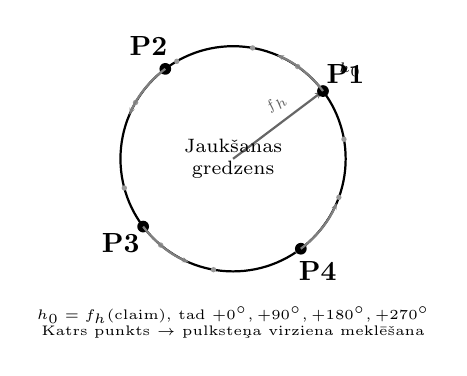
\begin{tikzpicture}[scale=0.65]
% Ring
\draw[thick] (0,0) circle (2.2cm);
% DID nodes on ring
\foreach \a in {10,55,80,120,150,195,230,260,305,340} {
  \fill[black!40] (\a:2.2) circle (1.5pt);
}
% Hash offset arrow pointing to initial position
\draw[-{Stealth[length=3pt]}, thick, black!60] (0,0) -- node[font=\tiny,above,sloped,pos=0.6] {$f_h$} (37:2.2);
\fill[black] (37:2.2) circle (2pt);
\node[font=\tiny,anchor=south west] at (37:2.35) {$h_0$};
% N=4 points offset from h0 by +0, +90, +180, +270
\foreach \offset/\l in {0/P1,90/P2,180/P3,270/P4} {
  \pgfmathsetmacro{\ang}{37+\offset}
  \node[fill=black, circle, inner sep=1.5pt] (p\offset) at (\ang:2.2) {};
  \node[font=\tiny,font=\bfseries] at (\ang:2.75) {\l};
  % clockwise search arc
  \draw[-{Stealth[length=2.5pt]}, thick, gray] (\ang:2.2) arc (\ang:\ang+30:2.2);
}
\node[font=\scriptsize, align=center] at (0,0) {Jaukšanas\\gredzens};
\node[font=\tiny, align=center] at (0,-3.2) {$h_0 = f_h(\text{claim})$, tad $+0^{\circ},+90^{\circ},+180^{\circ},+270^{\circ}$\\Katrs punkts $\rightarrow$ pulksteņa virziena meklēšana};
\end{tikzpicture}
\caption{Daudzpunktu atlase ($N{=}4$). Jaukšana $h_0$ nosaka nobīdi; 4 punkti vienmērīgi sadalīti no $h_0$.}
\label{fig:multipoint}
\end{figure}

\subsection{Liecinieka protokols}

\textbf{Liecinieka} loma nodrošina inkognito atbildību par verificētāja godīgumu caur kriptogrāfisku izaicinājuma koda protokolu:

\textbf{W1.\ solis.} Pieprasītājs paraksta verifikācijas pieprasījumu un nosūta to $N_w$ lieciniekiem---kontaktiem no pieprasītāja sociālā tīkla vai specializētiem liecinieku pakalpojumu sniedzējiem, kas darbojas par maksu.

\textbf{W2.\ solis.} Katrs liecinieks $w_i$ paraksta visu parakstīto pieprasījumu, saglabā oriģinālo parakstu $\sigma_i$ un aprēķina izaicinājuma kodu $c_i = h(\sigma_i)$. Izaicinājuma kods tiek pievienots pieprasījumam.

\textbf{W3.\ solis.} Pieprasījums, kas tagad nes $N_w$ izaicinājuma kodus, tiek nosūtīts verificētājam. Verificētājs novēro kodus, bet \emph{nevar noteikt}, kas ir liecinieki vai vai kodi atbilst reāliem parakstiem.

\textbf{W4.\ solis (godīgs verificētājs).} Ja verificētājs atbild atbilstoši savai deklarētajai politikai, izaicinājuma kodi paliek necaurspīdīgi. Liecinieki nekad netiek atklāti. Nekādi papildu dati netiek publicēti.

\textbf{W5.\ solis (politikas pārkāpums).} Ja verificētājs pārkāpj savu politiku (ignorē pieprasījumu, atbild nekonsekventi), pieprasītājs tur liecinieku oriģinālos parakstus $\sigma_i$. Tos var publicēt kā pavaddatus: jebkurš var verificēt $c_i = h(\sigma_i)$, pierādot, ka liecinieks bija klāt. Pieprasītājs var publicēt neatkarīgi---verificētājs jau ir parakstījis izaicinājuma kodus savā atbildē.

\textbf{Blefa īpašība.} Pieprasītājs dažiem vai visiem izaicinājuma kodiem var aizvietot nejaušas vērtības. Verificētājs nevar atšķirt īstus kodus (kurus balsta augstas reputācijas autoritātes) no trokšņa. Šī \emph{nenoteiktība} ir piespiešanas mehānisms: katrs pieprasījums nes risku, ka cienīta autoritāte to inkognito vēro. Šī spiediena uzturēšanas izmaksas ir tuvu nullei (nejaušu skaitļu ģenerēšana), kamēr negodīguma potenciālās izmaksas verificētājam ir katastrofālas. Godīga uzvedība tiek stimulēta pat tad, ja reālu liecinieku nav.

\textbf{Autoritāte kā liecinieks.} Autoritāte, kas apstiprina apgalvojumu, var apvienot liecinieka pakalpojumus: ,,Es apstiprinu tavu apgalvojumu un kalpoju kā inkognito liecinieks verifikācijas laikā.'' Tas ir dabisks biznesa modelis---autoritātei jau ir konteksts. Tomēr abas lomas ir loģiski neatkarīgas.

\subsection{Dārgā radikālisma princips}

Trīs izmaksu kanāli pastiprinās vienlaicīgi (att.~\ref{fig:radicalism}):

\textbf{1.\ kanāls: iterācijas izmaksas.} Katrs noraidījums piespiež jaunu iterāciju, kas patērē laiku un resursus. Lineāra izaugsme.

\textbf{2.\ kanāls: dokumenta uzblīšana.} Katra iterācija pievieno pilno verificētāja atbildi apgalvojuma dokumentam. Izaugsme ir lineāra, bet ar bāzes nobīdi: sākotnējā slodze (apgalvojuma saturs, autoritātes apstiprinājums, kriptogrāfiskie paraksti) jau ir ar netriviālu izmēru $B_0$. Kopējais izmērs pēc $k$ iterācijām: $S(k) = B_0 + k \cdot \Delta$, kur $\Delta$ ir vidējais atbildes izmērs.

\textbf{3.\ kanāls: verificētāja riska prēmija.} Risks ir subjektīvs. Verificētājs novērtē, vai pieprasošā DID deklarētās politikas ir pretrunā ar verificētāja paša komerciālajām, sociālajām vai politiskajām interesēm. Prēmija var eksponenciāli pieaugt līdz ar uztverto attālumu no verificētāja ,,ideāla'': $P(d) = \alpha \cdot e^{\beta d}$, kur $d$ ir verificētāja subjektīvā attāluma metrika. Aiz personiskās aizlieguma robežas verificētājs var atteikt pilnībā.

\begin{figure}[ht]
\centering
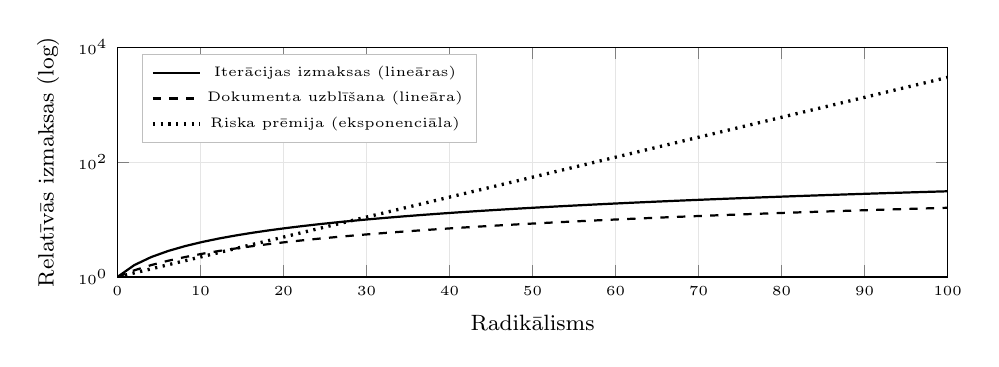
\begin{tikzpicture}
\begin{axis}[
    width=\columnwidth,
    height=4.5cm,
    xlabel={\footnotesize Radikālisms},
    ylabel={\footnotesize Relatīvās izmaksas (log)},
    ymode=log,
    xmin=0, xmax=100,
    ymin=1, ymax=10000,
    grid=major,
    grid style={gray!20},
    legend style={at={(0.03,0.97)},anchor=north west,font=\tiny,draw=gray!50},
    tick label style={font=\tiny},
    label style={font=\footnotesize},
]
\addplot[black, thick, domain=0:100, samples=50] {1 + 0.3*x};
\addlegendentry{Iterācijas izmaksas (lineāras)}
\addplot[black, thick, dashed, domain=0:100, samples=50] {1 + 0.15*x};
\addlegendentry{Dokumenta uzblīšana (lineāra)}
\addplot[black, thick, dotted, line width=1.2pt, domain=0:100, samples=100] {exp(0.08*x)};
\addlegendentry{Riska prēmija (eksponenciāla)}
\end{axis}
\end{tikzpicture}
\caption{Izmaksu eskalācija trijos kanālos. Riska prēmija dominē pie augsta radikālisma.}
\label{fig:radicalism}
\end{figure}

Būtiski, ka tā nav cenzūra. Neviens apgalvojums nav aizliegts. Sistēma cena risku (tab.~\ref{tab:costs}).

\begin{table}[ht]
\centering
\caption{Izmaksu salīdzinājums pa apgalvojumu tipiem.}
\label{tab:costs}
\footnotesize
\begin{tabular}{@{}lcccc@{}}
\toprule
\textbf{Tips} & \textbf{Iter.} & \textbf{Dok.} & \textbf{Maksa} & \textbf{Kopā} \\
\midrule
Ticams & $k_{\min}$ & $B_0$ & $P_{\min}$ & Zemas \\
Strīdīgs & $k_{\text{med}}$ & $B_0{+}k\Delta$ & $\alpha e^{\beta d}$ & Vidējas \\
Radikāls & $k_{\max}$ & $\gg B_0$ & $\gg P_{\min}$ & Ļoti augstas \\
Krāpniecisks & $\to\infty$ & --- & --- & Nepublicējams \\
\bottomrule
\end{tabular}
\end{table}

% ============================================================
% 6. REPUTATION AND RISK
% ============================================================
\section{Reputācija un riska novērtēšana}

\subsection{Reputācijas uzkrāšanas modelis}

Reputācijai ir trīs īpašības: \textbf{lēna uzkrāšana} (pakāpeniska izaugsme caur konsekventu uzvedību), \textbf{strauja iznīcināšana} (viena krāpšana var katastrofāli samazināt vērtējumu) un \textbf{individuāls novērtējums} (katra patērējošā puse var piemērot savu agregācijas funkciju).

\subsection{Reputablas autoritātes}

Reputabla autoritāte pārskata apgalvojumus un, ja apmierināta, tos līdzparaksta---liekot uz spēles savu reputāciju (att.~\ref{fig:authority}). Asimetrija ir apzināta: reputācijas iegūšana ir lēna (pakāpenisks $+\delta$ par godīgu apstiprinājumu), kamēr tās zaudēšana ir katastrofāla ($-\Delta \gg \delta$ par nepatiesu apstiprinājumu; ilustratīvi, piem., $+2\%$ pret $-70\%$). Optimālā stratēģija vienmēr ir noraidīt aizdomīgus apgalvojumus. Konkrētās $\delta$ un $\Delta$ vērtības ir sistēmas parametri.

\begin{figure}[ht]
\centering
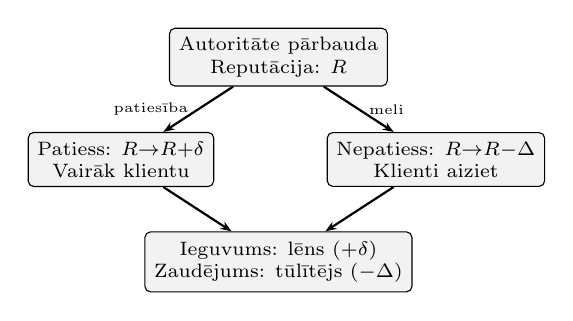
\begin{tikzpicture}[
    box/.style={draw, rounded corners=2pt, minimum width=2cm, minimum height=0.6cm, align=center, font=\scriptsize, fill=black!5},
    arr/.style={-{Stealth[length=4pt]}, thick}
]
\node[box] (exam) at (0,0) {Autoritāte pārbauda\\Reputācija: $R$};
\node[box] (true) at (-2,-1.3) {Patiess: $R{\to}R{+}\delta$\\Vairāk klientu};
\node[box] (false) at (2,-1.3) {Nepatiess: $R{\to}R{-}\Delta$\\Klienti aiziet};
\node[box] (insight) at (0,-2.6) {Ieguvums: lēns ($+\delta$)\\Zaudējums: tūlītējs ($-\Delta$)};

\draw[arr] (exam) -- node[left,font=\tiny] {patiesība} (true);
\draw[arr] (exam) -- node[right,font=\tiny] {meli} (false);
\draw[arr] (true) -- (insight);
\draw[arr] (false) -- (insight);
\end{tikzpicture}
\caption{Reputabla autoritāte---asimetriski stimuli.}
\label{fig:authority}
\end{figure}

\subsection{Daudzdimensionāla reputācija}

Reputācija nav skalārs, bet vektors vairākās dimensijās: finansiālā uzticamība, personiskā integritāte, profesionālā kompetence, pilsoniskā iesaiste un citas (att.~\ref{fig:reputation-radar}). Dažādi novērtēšanas pakalpojumu sniedzēji projicē šo vektoru atšķirīgi atkarībā no konteksta---aizdevējs par prioritāti izvirza finansiālo uzticamību, darba devējs profesionālo kompetenci, kaimiņš pilsonisko uzvedību. Nav vienota ,,pareiza'' reputācijas vērtējuma; ir tikai perspektīvas.

\begin{figure}[ht]
\centering
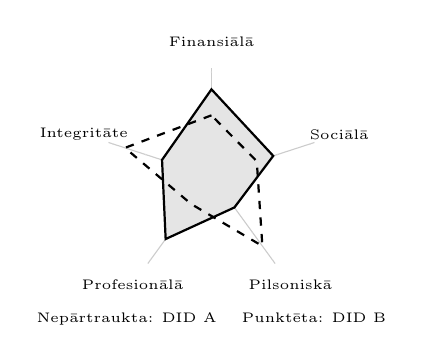
\begin{tikzpicture}[scale=0.55]
\foreach \a/\l in {90/Finansiālā,162/Integritāte,234/Profesionālā,306/Pilsoniskā,18/Sociālā} {
  \draw[gray!40] (0,0) -- (\a:2.5);
  \node[font=\tiny, align=center] at (\a:3.1) {\l};
  \foreach \r in {0.8,1.6,2.4} {
    \fill[black!15] (\a:\r) circle (0.5pt);
  }
}
\draw[thick, fill=black!10] (90:2.0) -- (162:1.2) -- (234:1.8) -- (306:0.9) -- (18:1.5) -- cycle;
\draw[thick, dashed] (90:1.4) -- (162:2.1) -- (234:0.8) -- (306:2.0) -- (18:1.1) -- cycle;
\node[font=\tiny] at (0,-3.3) {Nepārtraukta: DID A \quad Punktēta: DID B};
\end{tikzpicture}
\caption{Daudzdimensionāli reputācijas vektori. Dažādi DID uzrāda atšķirīgus profilus pa dimensijām.}
\label{fig:reputation-radar}
\end{figure}

\subsection{Demokratizēta riska novērtēšana}

RSN demokratizē sistemātisku riska novērtēšanu---spēju, kas pašlaik ir koncentrēta finanšu institūcijās, taču piemērojama tālu ārpus banku sfēras. Rūpniecības konglomerāti, kas novērtē piegādātāju uzticamību, apdrošināšanas sabiedrības, kas cena uzvedības risku, uzticamības pārbaude apvienošanās un pārņemšanas darījumos, iekārtu kalpošanas laika novērtēšana ražošanā---visur, kur darījuma partnera risks prasa novērtēšanu, RSN nodrošina decentralizētu, uz tirgu balstītu alternatīvu. Interpretācijas pakalpojumu tirgus pārvērš neapstrādātus daudzdimensionālus reputācijas datus rīcībai izmantojamos kopsavilkumos, padarot darījuma partnera novērtēšanu pieejamu jebkuram dalībniekam par robežizmaksām.

% ============================================================
% 7. CONSENSUS AND DISPUTE RESOLUTION
% ============================================================
\section{Konsenss un strīdu izšķiršana}

\subsection{Decentralizēta taisnīguma modelis}

RSN pārformulē taisnīgumu kā divpusēju sarunu problēmu. Draudi ar pastāvīgu, verificējamu reputācijas kaitējumu ir efektīvāks attur\-oša faktors nekā tiesvedība, ko cietusī puse nevar atļauties.

\subsection{Emerģents konsenss}

Katrs dalībnieks uztur personisku gandarījuma slieksni. Tīkla kopējais konsenss rodas kā tūkstošiem divpusēju sarunu statistiskais vidējais (att.~\ref{fig:consensus}). Atbilde tālu virs konsensa (barbariska) ir dārgi publicējama. Atbilde tuvu konsensam (samērīga) ir lēta. Konsenss nav noteikums---tas ir cenas signāls.

\begin{figure}[ht]
\centering
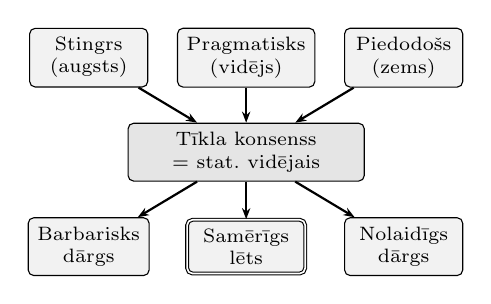
\begin{tikzpicture}[
    person/.style={draw, rounded corners=2pt, minimum width=1.5cm, minimum height=0.5cm, align=center, font=\scriptsize, fill=black!5},
    arr/.style={-{Stealth[length=4pt]}, thick}
]
\node[person] (a) at (-2,0) {Stingrs\\(augsts)};
\node[person] (b) at (0,0) {Pragmatisks\\(vidējs)};
\node[person] (c) at (2,0) {Piedodošs\\(zems)};
\node[person, fill=black!10, minimum width=3cm] (cons) at (0,-1.2) {Tīkla konsenss\\= stat.\ vidējais};
\node[person] (exp) at (-2,-2.4) {Barbarisks\\dārgs};
\node[person, double] (prop) at (0,-2.4) {Samērīgs\\lēts};
\node[person] (neg) at (2,-2.4) {Nolaidīgs\\dārgs};

\draw[arr] (a) -- (cons);
\draw[arr] (b) -- (cons);
\draw[arr] (c) -- (cons);
\draw[arr] (cons) -- (exp);
\draw[arr] (cons) -- (prop);
\draw[arr] (cons) -- (neg);
\end{tikzpicture}
\caption{Emerģents konsenss no individuāliem gandarījuma sliekšņiem.}
\label{fig:consensus}
\end{figure}

\subsection{Soda kalibrēšana}

Katrs DID turētājs publiski deklarē atbildes uz konkrētām nekrietnības kategorijām. Nesamērīgi bargas vai iecietīgas deklarācijas piesaista negatīvus reputācijas signālus. Samērīgas deklarācijas tiek pieņemtas bez berzes---paškalibrējoša soda sistēma.

Konsensa deklarācijas pašas ir pakļautas liekulības atklāšanai: deklaratīvi apņemties par konsensa pozīciju, uzvedoties nekonsekventi, ir reputācijas pārkāpums, kas ir smagāks par pašu novirzi, jo tas demonstrē tīšu maldināšanu.

\subsection{Deleģēšana}

Visas aktivitātes DID ietvaros---ar vienu izņēmumu---var deleģēt citam DID. \textbf{Subjekta loma---DID, par kura uzvedību ir apgalvojums---nav deleģējama; tā ir nepārnesami piesaistīta identitātes turētājam, uz kuru apgalvojums attiecas.} Pārējās aktīvās lomas---Izdevējs, Autoritāte, Liecinieks, Verificētājs---var nodot norādītam delegāta DID, vai tas būtu verifikācijai, apgalvojuma iesniegšanai, dalībai konsensā vai strīdu izšķiršanai. Deleģēšana ir atsaucama jebkurā laikā. Tas dara iespējamu specializāciju (piem., profesionālus verifikācijas pakalpojumus), kamēr turētājs saglabā galīgo kontroli un atbildību. Deleģēšana attiecas uz visu sistēmu un ir būtiska mērogojamībai.

\subsection{No individuālas morāles uz emerģentu sabiedrisko līgumu}

Katra DID deklarētā politika ir individuālas morāles formalizācija: ko turētājs uzskata par pieņemamu, kā tas reaģē uz konkrētu uzvedību, ko tas prasa no darījuma partneriem. Šīs politikas neuzspiež sistēmas projektētājs---tās izvēlas katrs dalībnieks un izsaka mašīnlasāmā formā.

Šī formalizācija dara iespējamu trīs posmu emerģenci. Pirmkārt, individuālā morāle tiek kodēta kā \textbf{politika}---deklarētu noteikumu, sliekšņu un atbildes funkciju kopa, kuru DID apņemas ievērot. Otrkārt, visu politiku kopums tīklā rada \textbf{emerģentu ētiku}---statistiski novērojamas normas, kuras neveidoja neviens atsevišķs dalībnieks, bet kuras rodas no tūkstošiem individuālu morālu pozīciju mijiedarbības~\cite{durkheim1893}. Treškārt, šī emerģentā ētika, izteikta kā kopīgas uzvedības normas, ko piespiež caur divpusējiem cenas signāliem, veido \textbf{izmērāmu sabiedrisko līgumu}---nevis teorētisku konstruktu, ko neviens nav parakstījis~\cite{rawls1971}, bet empīriski novērojamu noteikumu kopu, ko balsta faktiskā uzvedība.

Šis process atspoguļo morālo pamatu teorijas atziņas~\cite{haidt2012}: cilvēka morāle ir intuitīva, plurālistiska un kultūrai mainīga. RSN neprasa morālu konsensu kā ievadi; tas rada uzvedības konsensu kā izvadi. Iegūtais sabiedriskais līgums nav statisks---tas attīstās, dalībniekiem pievienojoties, aizejot un pielāgojot savas politikas atbildē uz tīkla atgriezenisko saiti. Atšķirībā no klasiskās sabiedriskā līguma teorijas šis līgums ir atsaucams, novērojams un piespiežams bez suverēna.

% ============================================================
% 8. ECONOMIC MODEL
% ============================================================
\section{Ekonomiskais modelis}

Iepriekšējās sadaļas aprakstīja rīku---RSN verifikācijas mehānismus, izmaksu struktūru un emerģentu konsensu. Šī sadaļa apraksta metodoloģiju šī rīka pielietojumam fiskālajā un pārvaldes pārejā. Rīks ir vispārējas nozīmes; zemāk aprakstītā metodoloģija ir viens iespējams pielietojums.

\subsection{Stimulu struktūra}

Reputācija kā kapitāls rada tiešus stimulus godīgai uzvedībai. Normālā darbībā dalībnieki dabiski veido reputāciju caur ikdienas darījumiem un izpildītām saistībām. Galvenie izdevumi ir par \emph{negatīviem} apgalvojumiem---citu nodarītā kaitējuma reģistrēšanu. Šī asimetrija stimulē noderīgu, uzticamu uzvedību: būt godīgam neizmaksā neko papildus, kamēr būt kaitīgam rada dokumentētu pēdu, kuru citi maksās, lai saglabātu. Liekulība---deklarēt noteikumus, tos neievērojot---ir vis\-dārgākais neveiksmes veids, jo tā demonstrē tīšu maldināšanu.

\subsection{Paralēla fiskālā sistēma}

Trīs komponenti rada konkurences spiedienu: (1)~\textbf{Vienkāršs nodoklis}---viena proporcionāla likme bez izņēmumiem, sākotnēji nedaudz zem esošās efektīvās likmes; (2)~\textbf{Elektroniska izdevumu reģistrācija (ESR)}---apvēršot Čehijas EET modeli tā, lai pilsoņi uzraudzītu valsts izdevumus; (3)~\textbf{Pilsoņu virzīta nodokļu sadale}---sākot ar dažiem procentiem pirmajā gadā un sasniedzot pēc desmit gadiem jebko no zemām divciparu vērtībām līdz pilnīgai migrācijai uz pilsoņu virzītu sistēmu atkarībā no ieviešanas ātruma. Faktiskais temps ir atkarīgs no ātruma, kādā rodas brīvā tirgus alternatīvas valsts pakalpojumiem, un no valsts gatavības sadarboties ar pāreju; laika funkcijai nav jābūt lineārai, un nav iemesla noteikt augšējo robežu tam, kur ieviešana galu galā var nonākt.

% ============================================================
% 9. MIGRATION PATH
% ============================================================
\section{Migrācijas ceļš}

Migrācija notiek caur trim fāzēm (att.~\ref{fig:migration}): \textbf{1.\ fāze: pārklājums} (RSN kā informatīvs slānis, valsts ir vienīgais sniedzējs), \textbf{2.\ fāze: konkurence} (RSN nodrošina funkcionālas alternatīvas, divsistēmu lietošana) un \textbf{3.\ fāze: pāreja} (RSN pārspēj valsts ekvivalentus, brīvprātīga migrācija). Pāreja ir atgriezeniska katrā posmā.

\begin{figure}[ht]
\centering
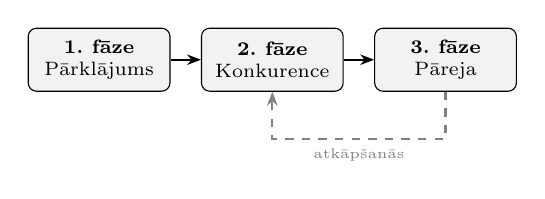
\begin{tikzpicture}[
    phase/.style={draw, rounded corners=3pt, minimum width=1.8cm, minimum height=0.8cm, align=center, font=\scriptsize, fill=black!5},
    arr/.style={-{Stealth[length=5pt]}, thick}
]
\node[phase] (p1) at (0,0) {\textbf{1.\ fāze}\\Pārklājums};
\node[phase] (p2) at (2.2,0) {\textbf{2.\ fāze}\\Konkurence};
\node[phase] (p3) at (4.4,0) {\textbf{3.\ fāze}\\Pāreja};

\draw[arr] (p1) -- (p2);
\draw[arr] (p2) -- (p3);
\draw[arr, dashed, gray] (p3.south) -- ++(0,-0.6) -| node[below,font=\tiny,pos=0.25] {atkāpšanās} (p2.south);
\end{tikzpicture}
\caption{Trīs fāžu migrācija---atgriezeniska katrā posmā.}
\label{fig:migration}
\end{figure}

Galvenais spiediena mehānisms ir fiskāls: kad nosacītie nodokļu maksātāji sasniedz ,,ekonomiski nozīmīgu mazākumu $X$''---grupu, kas ir pietiekami liela, lai represijas pret to radītu netriviālu ekonomisku kaitējumu un pilsoniskā nepaklausība kļūtu par ticamu draudu---valsts uzsāk sarunas. Ilustrācijai izmantojam $X \approx 15\%$ no IKP, taču faktiskais slieksnis ir atkarīgs no konkrētās ekonomikas.

% ============================================================
% 10. SECURITY ANALYSIS
% ============================================================
\section{Drošības analīze}

Mēs apsveram piecas pretinieku kategorijas: individuāli ļaunprātīgi dalībnieki, organizētas grupas, korporatīvi pretinieki, valsts līmeņa pretinieki un protokola līmeņa pretinieki.

\textbf{Sibilas noturība}~\cite{douceur2002}. Reputācijas veidošana prasa ilgstošu, verificējamu mijiedarbību. Veiksmīga Sibilas uzbrukuma izmaksas aug lineāri līdz ar viltus identitātēm un kvadrātiski līdz ar mērķa reputācijas līmeni. Vairāku DID darbināšana paralēli ir iespējama, bet apzināti dārga---katrai identitātei neatkarīgi jāuzkrāj reputācija caur patiesu aktivitāti. Brīvās sabiedrībās šīs izmaksas attur no gadījuma rakstura ļaunprātības; diktatūrās paralēlie DID kļūst par izdzīvošanas rīku, kas dara iespējamu nodalītu pretošanos, pagrīdes koordināciju un drošāku melnā tirgus navigāciju.

\textbf{Aizsardzība pret slepenu vienošanos.} Savstarpējas apstiprināšanas modeļi slēgtu grupu ietvaros ir atklājami caur sociālā grafa analīzi. Reputācijas agregācijas funkcijas atlaiž apgalvojumus no cieši saistītiem avotiem.

\textbf{Valsts līmeņa pretinieks.} Sīpola maršrutēšana, centralizētas infrastruktūras neesamība un Verificētāja lomas sadale pa dalībnieku bāzi nodrošina, ka apspiešana prasa pasākumus, kas ir nesamērīgi ar jebkādu ieguvumu.

\textbf{Privātums pret atbildību.} Pseidonimitāte---vidusceļš starp anonimitāti un identitātes atklāšanu---ļauj DID uzkrāt jēgpilnu reputāciju, neatklājot turētāja reālās pasaules identitāti.

% ============================================================
% 11. PRIVACY
% ============================================================
\section{Privātuma apsvērumi}

RSN privātuma modelis balstās uz pseidonimitāti. Turētājs kontrolē identitātes atklāšanu: minimālu (tīrs pseidonīms), selektīvu (saistīti konkrēti akreditācijas dati) vai pilnu (piesaistīta juridiskā identitāte). Publicētie apgalvojumi ir pastāvīgi---sistēma atbalsta kontekstuālu labošanu, bet ne dzēšanu. Turētājs var pamest kompromitētu DID un sākt no jauna, atsakoties no uzkrātās reputācijas.

% ============================================================
% 12. RELATED WORK
% ============================================================
\section{Saistītie darbi}

W3C DID Core specifikācija~\cite{did2022} un Ceramic Network~\cite{ceramic2023} nodrošina identitātes pamatu. EigenTrust~\cite{kamvar2003} demonstrēja izkliedētu reputācijas agregāciju bez centrālas autoritātes. SBT~\cite{weyl2022} ieviesa nepārnesamus sociālos žetonus. RSN atšķiras ar uzsvaru uz ekonomiskajām izmaksām kā kvalitātes filtru un ar mehānismu radikālisma cenošanai.

DAO~\cite{buterin2014} un kvadrātiskā balsošana~\cite{buterin2019} demonstrēja decentralizētas pārvaldes iespējamību. RSN atvasina konsensu no divpusējām cenu sarunām, nevis no balsošanas.

Priekšlikums balstās uz anarhokapitālisma teoriju~\cite{rothbard1973,hoppe2001} attiecībā uz privātu pakalpojumu sniegšanu, taču atšķiras divos būtiskos aspektos: tas ir projektēts ļaunprātībai un atriebīgiem impulsiem, nevis pieņem racionalitāti, un tas ierosina pakāpenisku pāreju, nevis revolūciju. Emerģentu sabiedrisko līgumu jēdzienam ir priekšteči Haijeka spontānās kārtības teorijā~\cite{hayek1973}.

\textbf{Anarhoagorisms.} RSN dala ievērojamu kopīgu pamatu ar agorisma pretekonomiku~\cite{konkin2006}---īpaši uzsvaru uz paralēlu institūciju veidošanu un brīvprātīgu apmaiņu. Tomēr agorisms mēdz pieņemt racionālu paš\-interesi kā pietiekamu koordinācijas mehānismu un bieži trūkst konkrēta migrācijas ceļa no esošajām valsts struktūrām. RSN skaidri iekļauj neracionālas uzvedības tieksmes un nodrošina fiskālā spiediena mehānismu pakāpeniskai pārejai.

\textbf{Meritokrātija.} RSN var būt pirmais funkcionālais apraksts tam, kā meritokrātija~\cite{young1958} var rasties kā sistēmiska īpašība, nevis kā sauklis. Tradicionālās meritokrātiskās sistēmas neizdodas, jo tām nepieciešama centrāla autoritāte, lai definētu un piespiestu ,,nopelnu''. RSN nopelni rodas no divpusējiem novērtējumiem: tie, kas sniedz vērtību, uzkrāj reputāciju; neviena komiteja neizlemj, kam ir nopelni.

\textbf{Īpašums kā privilēģija.} RSN fundamentāli atkāpjas no anarhokapitālisma un austriešu skolas traktējuma par īpašumtiesībām kā dabiskām un absolūtām. RSN ietvarā īpašums ir \emph{privilēģija}---sociāla atzīšana, ko galējos gadījumos kopiena var atsaukt, kad dalībnieks fundamentāli pārkāpj kopīgas normas (nodevība, atteikšanās aizstāvēt kopienu eksistenciālā krīzē, sistemātiska ekspluatācija). Tā nav valsts ekspropriācija, bet sociālas atzīšanas atsaukšana no divpusēju attiecību tīkla.

% ============================================================
% 13. LIMITATIONS
% ============================================================
\section{Diskusija un ierobežojumi}

\textbf{Aukstais starts.} RSN vērtība ir atkarīga no tīkla efektiem; agrīnie ieviesēji saskaras ar ierobežotu vērtību, līdz dalība sasniedz slieksni. Tomēr pat no agrīnajiem posmiem DID tīkls kalpo kā noderīgs papildu informācijas avots. Sagaidāms, ka agrīnā reputācijas novērtēšana un autoritāšu novērtēšana attīstīsies pakāpeniski, pieaugot sarežģītībai.

\textbf{Pretpiesūkšanās un piekļuves kontrole.} Mērķa DID var uzlikt pakāpeniskas maksas un piekļuves ierobežojumus pieprasījumiem no zemas reputācijas DID. Tā nav bināra, bet nepārtraukta skala: jo mazāk reputācijas ir pieprasošajam DID, jo mazāk informācijas tas saņem, jo ilgāk tas gaida un jo vairāk maksā. Šis mehānisms stimulē patiesu dalību pār pasīvu patēriņu.

\textbf{Piekļuves nevienlīdzība.} Apgalvojumu publicēšanas izmaksas var filtrēt leģitīmas sūdzības no ekonomiski nelabvēlīgā stāvoklī esošiem dalībniekiem. Mazināšana: katrs dalībnieks vienlaikus kalpo kā potenciāls verificētājs (vai deleģē šo lomu) un pelna verifikācijas maksas. Pietiekami ilgā laika horizontā neradikālam dalībniekam vajadzētu tuvoties finansiālai neitralitātei---verifikācijas ieņēmumiem aptuveni kompensējot publicēšanas izmaksas. Tā ir statistiska gaidāmā vērtība, nevis garantija.

\textbf{Reputācijas nevienlīdzība.} Agrīnie ieviesēji uzkrāj priekšrocības, kas var radīt barjeras vēlākiem pievienotājiem. Tomēr reputācijas novērtēšanu veic trešo pušu sniedzēji, kas var izvēlēties mazināt pirmā gājēja priekšrocību caur savām agregācijas algoritmiem. Būt pirmajam ar labu reputāciju ir leģitīma salīdzinoša ekonomiska priekšrocība---un tā ir apzināta.

\textbf{Atklātie jautājumi.} Optimālas izmaksu funkcijas, agregācijas standarti, protokola pārvalde un mijiedarbība ar mākslīgā intelekta ģenerētiem sintētiskiem reputācijas datiem paliek nākotnes darba jomas.

Šis raksts neapgalvo, ka RSN radīs optimālus rezultātus visos apstākļos. Tas apgalvo, ka RSN ir \emph{īstenojama} alternatīva---tehniski ieviešama, ekonomiski paš\-uzturoša un sociāli saderīga ar cilvēka uzvedības tieksmēm tādām, kādas tās patiesībā ir.

% ============================================================
% 14. CONCLUSION
% ============================================================
\section{Secinājums}

Šis raksts ir prezentējis reputācijas sociālo tīklu---decentralizētu protokolu, kas dara iespējamu pseidonīmu, verificējamu reputācijas apmaiņu. Dārgā radikālisma princips nodrošina, ka krāpnieciski apgalvojumi tiek izcenoti no aprites bez cenzūras. Ierosinātais migrācijas ceļš dara iespējamu pakāpenisku, atgriezenisku pāreju no esošajām institūcijām. Projekts iekļauj cilvēka dabu tādu, kāda tā ir---ieskaitot sīkumainību, ļaunprātību un vēlmi pēc atriebīga gandarījuma---, nevis prasa ideoloģisku transformāciju. Rezultāts nav utopija, bet sistēma, kurā taisnīgums ir pieejams, reputācija ir nopelnīta un nekrietnības izmaksas nes tā puse, kas tās izraisīja.

% ============================================================
% REFERENCES
% ============================================================
\bibliography{references}

\end{document}
